\section{Visioner om den samlede forandring}
I dette afsnit beskrives projektgruppens forslag tilforbedringer af MinSP. Beskrivelsen er med udgangspunkt i MUST-metodens princip om samlede vision.\\
Udover en beskrivelse af den tekniske løsning af forbedringsforslagene har vi derfor også indraget en vurdering og beskrivelse af hvordan ændringerne vil påvirke arbejdsorganisering og hvilke konsekvenser det vil få for sundhedspersonalet. \\
Endelig indgår også en vurdering af hvilke kvalifikationsbehov ændringerne evt. vil medføre.
%I dette afsnit ser vi på hvordan visionerne om den samlede forandring, forankres i Regions Sjællands eksisterende version af it-systemet MinSP, dvs. hvordan visionerne skal integreres og anvendes af patienter og sundhedspersonale. \footnote{Professionel it-forundersøgelse, Bødker, Kensing, Simonsen, s. 211} 
\subsection{Teknologi}
%
% ! ER Diagram over de nye funktionalitere / visioner
%
\subsubsection{It-systemer og it-platform}
It-platformen for den samlede vision for MinSP er Sundhedsplatformen.
\\\\
\textbf{Prioritet 1, Receptfornyelse} \\
It-systemerne er udover MinSP også Sundhedsplatformen og muligvis apotekernes systemer og FMK (det fælles medicin kort), da der skal være integration i mellem disse systemer.
\\\\
\textbf{Prioritet 2, Samling af al information} \\
%
% ? - Anders Lassen: "Læring og videnscenter. Der er allerede patienthåndbogen Jeg tror det er out-of-scope":
%
Vores visioner er, at denne funktionalitet vil kunne løses med en 'standardløsning', da der allerede eksisterer flere troværdige informationssider, hvor det er læger, der vedligeholder siderne. \\
Viden og information om diabetes kan slås op i 'Patienthåndbogen'. Der findes allerede et link til 'Patienthåndbogen' i MinSP, men dette ligger 'gemt' i undermenuen 'Historik' under hovedmenuen 'Sundhedsdata'.
\\ \\
Under en menu 'Information om dine Diagnoser', kunne et link til 'Patienthåndbogen' placeres. \\
I samme menu kan der lægges et link til 'Diabetesforeningen', der tilbyder fællesskab mellem diabetikere i form af f.eks. motivationsgrupper og diabetescaféer samt rådgivning til diabetikere.
\\
Endvidere kan et link til 'Steno Diabetes Center' give video-information omkring f.eks. 'Hvordan man måler blodglukose', en diætist der fortæller om 'Kulhydrattælling' og informerer om kost og motion. og en overlæge der fortæller om 'Graviditetsdiabetes' m.fl. \\
På siden er der også information om blandt andet det at være ny med diabetes, til gravide med diabetes, hjælp til at forstå tal, madopskrifter og meget meget mere. 
\\ \\
Disse 'standardløsninger' kan være en måde til at løse funktionaliteten 'Samling af al information', og dermed undgås en dyr løsning, hvor hospitalernes sundhedspersonale skal vedligeholde egen udviklede informationssider på MinSP.
\\\\
\textbf{Prioritet 3, Uniforme Prøvesvar} \\
It-systemerne er udover MinSP også Sundhedsplatformen og FMK, da der skal være integration i mellem disse systemer.
\subsubsection{Funktion}  
% ? - Indenholde: 'Liste over de enkle it-systemers funktioner'
\textbf{Prioritet 1, Receptfornyelse}\\
Receptfornyelse er en funktionalitet, der skal ny-udvikles, da visionen er at det skal være integrere i MinSP og Sundhedsplatformen. Kravet til funktionaliteten skal være, så patienter, i MinSP, selv kan aktivere fornyelse af en eller flere recepter for deres ordinerede medicin. 
\\
Receptfornyelsen skal være synlig og skal derfor placeres som en hovedmenu øverst på MinSP. Undermenuen til hovedmenuen 'Receptfornyelse' skal indeholde: 'Forny recept', 'Medicin kort' og 'Historik'.
\\
Man skal kunne følge gangen i receptfornyelsen fra status 'Medicin bestilt' til 'Medicin kan hentes på apoteket'. Man skal også kunne vælge modtager-apotek, med to valgmuligheder, samt om man ønsker en påmindelse om receptfornyelse og i hvilken form (sms, besked i app'en, privat mail eller eboks). 
\\ 
Recept skal kun kunne fornys, når sidst udleverede dosis er ved slippe op.  
\\
'Medicinkortet' skal indeholde en liste over ordineret medicin.\\ 
'Historik' skal indeholde en liste over alle udleveringer af medicin til dato.
\\ \\
Vi vurderer, at 'Receptfornyelse' er en kompliceret funktionalitet, da den skal ny-udvikles, og da der ikke er noget eksisterende funktionalitet, der kan genbruges. Funktionaliteten er også kompliceret, fordi sikkerheden skal være høj i forhold til, at der ikke må udleveres for meget medicin, og da det kun er den ordinerede medicin, der må fornys. \\
Udviklingen af statuslinje, for gangen i receptfornyelsen, vil også være kompliceret, fordi registreringen skal overføres af sundhedspersonalet fra Sundhedsplatformen til MinSP.\\
Modtagerapotek skal kunne vælges i forhold til bopæl, og det vurdere vi også vil være kompliceret, fordi der skal bruges data omkring hvor alle apoteker i Region Sjælland ligger.\\
Påmindelse vil kræve, at der beregnes en dato for fornyelse af recept i forhold til sidste fornyelse. Hertil skal bruges databaser med oplysninger om om ordineret medicin, historikken for udleveret medicin og receptfornyelser. Vi forudsætter at databaser med disse oplysninger allerede findes, men at der skal laves integration med disse databaser.\\
I databasen for MinSP skal Patient tabellen udvides til at kunne gemme oplysninger om 'Primær apotek' og 'Sekundær apotek'.
\\\\
\textbf{Prioritet 2, Samling af al information} \\
Et forslag til at imødekomme visionen om en 'Samling af al information' kunne være, at under hovedmenuen Profil, at tilføje en undermenu 'Information om dine diagnoser'. Under denne undermenu kan der placeres link til f.eks. Patienthåndbogen, Diabetesforeningen og Steno Diabetes Center.
\\\\ 
\textbf{Prioritet 3, Uniforme Prøvesvar} \\
Denne funktionalitet vil kunne løses ved, at man til hvert enkelt prøvesvar knytter en forklaring af prøve-typen på dansk. Der skal her udover angives, hvor prøven er taget (navn på hospital, læge eller laboratorie).\\
Prøvesvarene skal holdes adskilt pr. diagnoses, hvis patienten har flere diagnoser.\\
I databasen for MinSP skal tabel med prøvesvar udvides til at kunne gemme forklarende tekst på dansk, om hvad prøven viser, navn på hospital / læge / laboratorie, hvor prøven er taget. Derfor skal der også oprettes en tabel med hospitals- / læge- / laboratorie navne, som navnet kan hentes fra.\\ 
Tekstbeskrivelsen kan være en standard tekst pr. prøvetype, men navet på stedet, hvor prøven er taget, kan variere. Dette skal derfor indrapporteres af personalet, når prøvesvar indrapporteres. \\
For at kunne holde prøvesvar adskilt pr. diagnose, skal tabellen med prøvesvar, i databasen for MinSP, udvides til at kunne gemme oplysninger om diagnose. Sundhedspersonalet skal, for hvert prøvesvar, indrapportere relevant diagnose for prøvesvaret. 
\subsubsection{Brugergrænseflader} % Krav til Brugergrænseflader
Brugergrænsefladerne skal designes så de overholder GUI-guidelines for god interaktions design. %  Benyon s. 88 
\\\\
\textbf{Prioritet 1, Receptfornyelse} \\
Implementering af receptfornyelses funktionaliteten vil kræve integration med Sundhedsplatformens medicinmodul og apotekerenes systemer. 
Der skal være en ny grænseflade mellem MinSP og FMK.\\\\
Forslag til brugergrænseflade for patienten fremgår af nedenstående Mock-up's:\\
\begin{figure}[H]
	\centering
	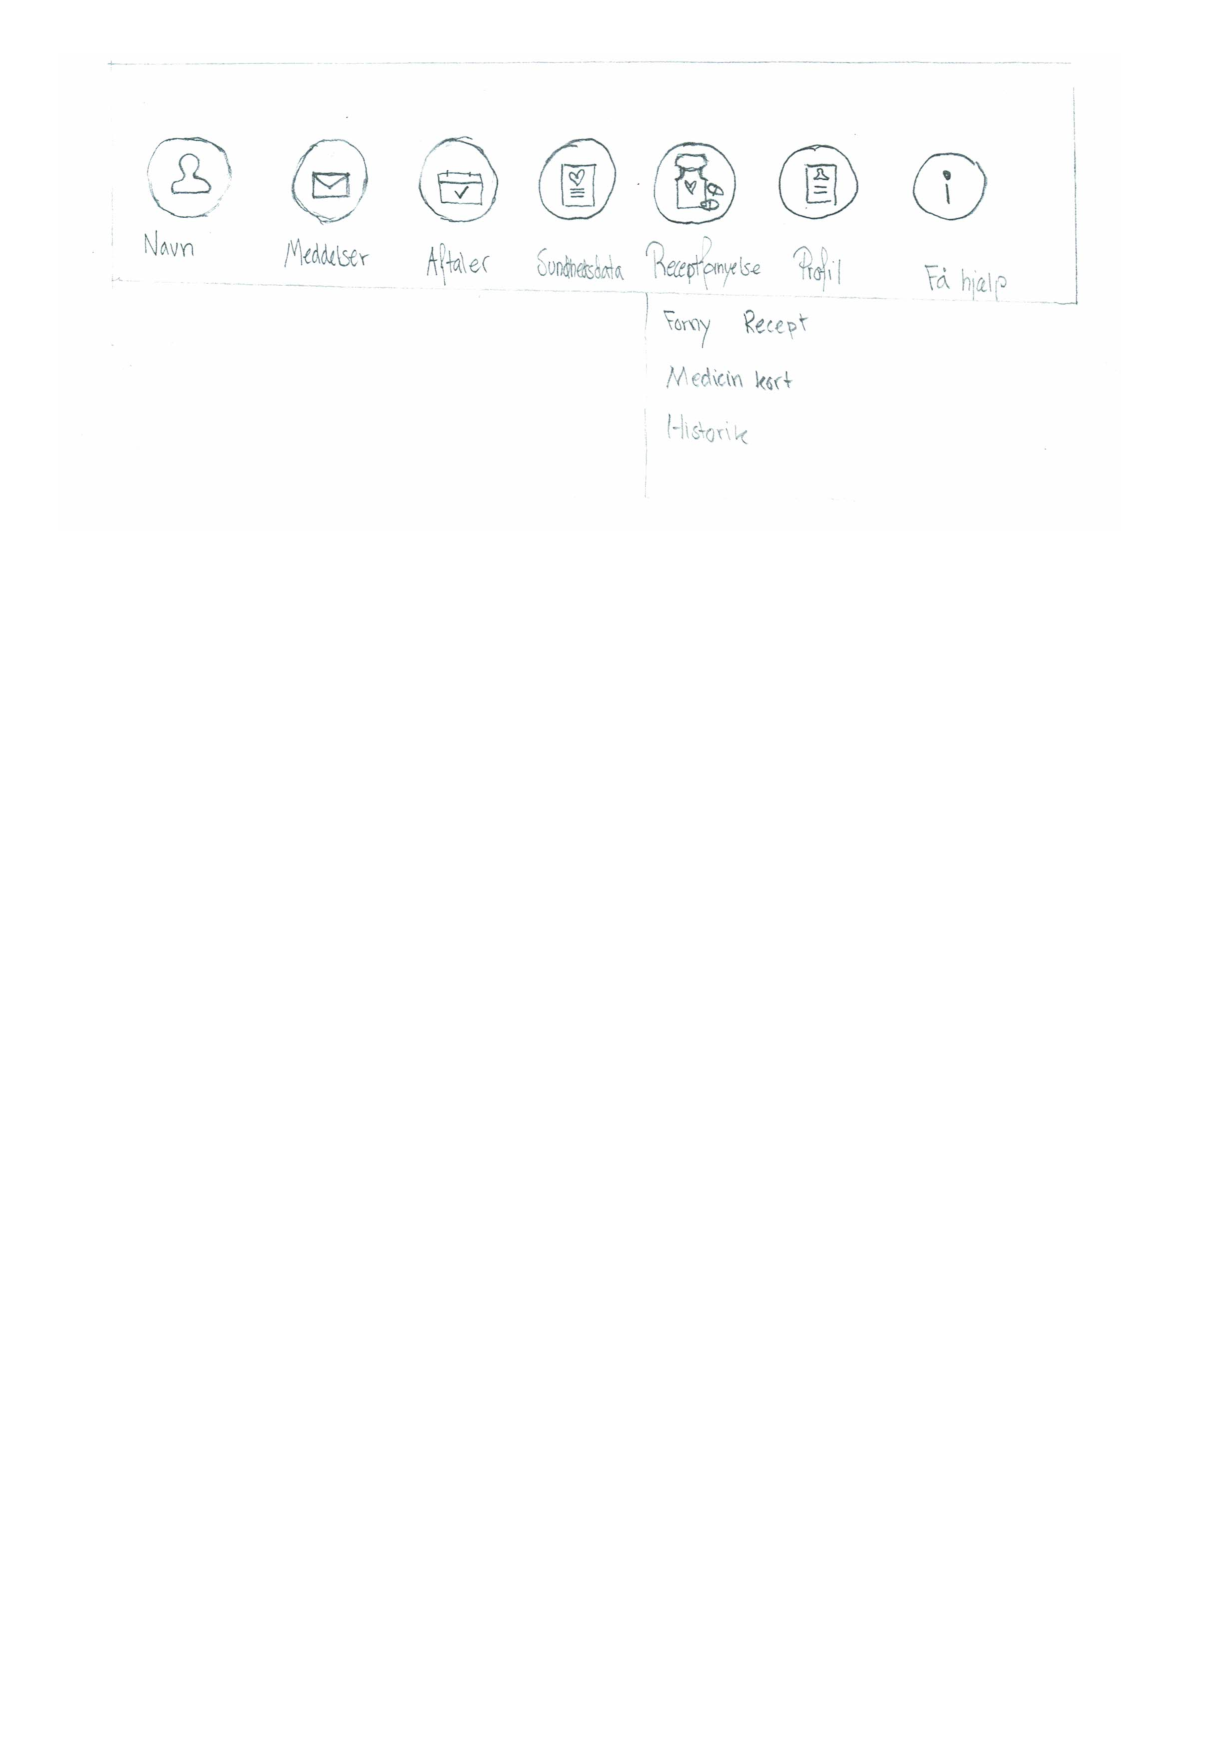
\includegraphics[angle=0, height=0.36\textheight]{Materials/FornyRecept_Hovedmenu.pdf}
	\caption{Mock-up for modulet 'Receptfornyelse': Hovedmenuen}
	\label{fig:Mock-Up}
\end{figure}
\begin{figure}[H]
	\centering
	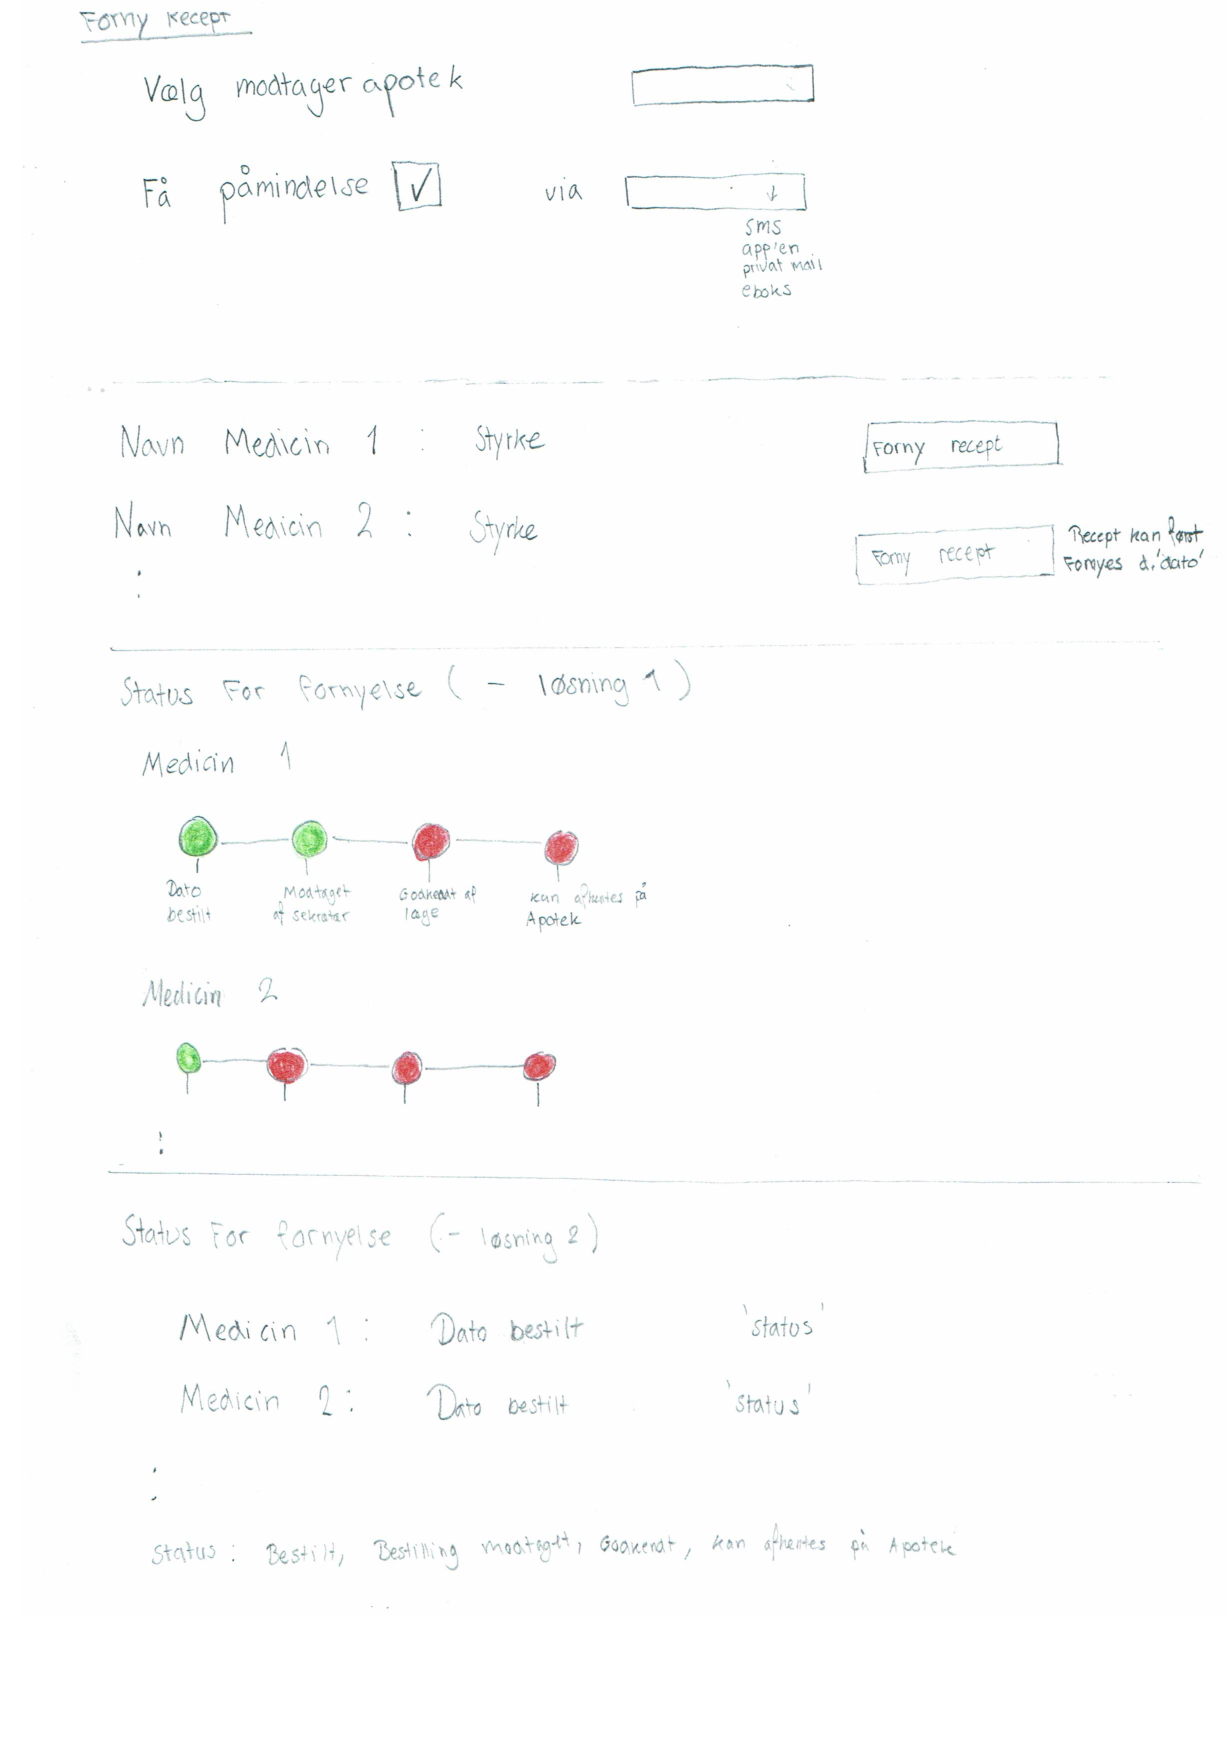
\includegraphics[angle=0, height=0.85\textheight]{Materials/FornyRecept.pdf}
	\caption{Mock-up for modulet 'Receptfornyelse': Undermenu, 'Forny recept'}
	\label{fig:Mock-Up}
\end{figure}
I 'Vælg modtagerapotek' skal man i en drop-down menu kunne vælge mellem de to apoteker tættest på en.\\
Bemærk at knappen 'Forny recept' skal være blokkeret i perioden hvor recept ikke må fornys. Der skal udover indformeres om hvornår patienten kan forny sin recept.\\
Når patienten fornyer sin recept skal være en fortrydelses besked: 'Er du sikker på du vil forny din recept?' Hvor man skal kunne vælge 'ja' eller 'nej'. Dette kan evt. laves som en pop-up. \\
Der er to forslag til måden status for fornyelse kan vises på. Status mulighederne i løsning to er: Bestilt, bestilling modtaget, godkendt og kan afhentes på Apotek.\\
\begin{figure}[H]
	\centering
	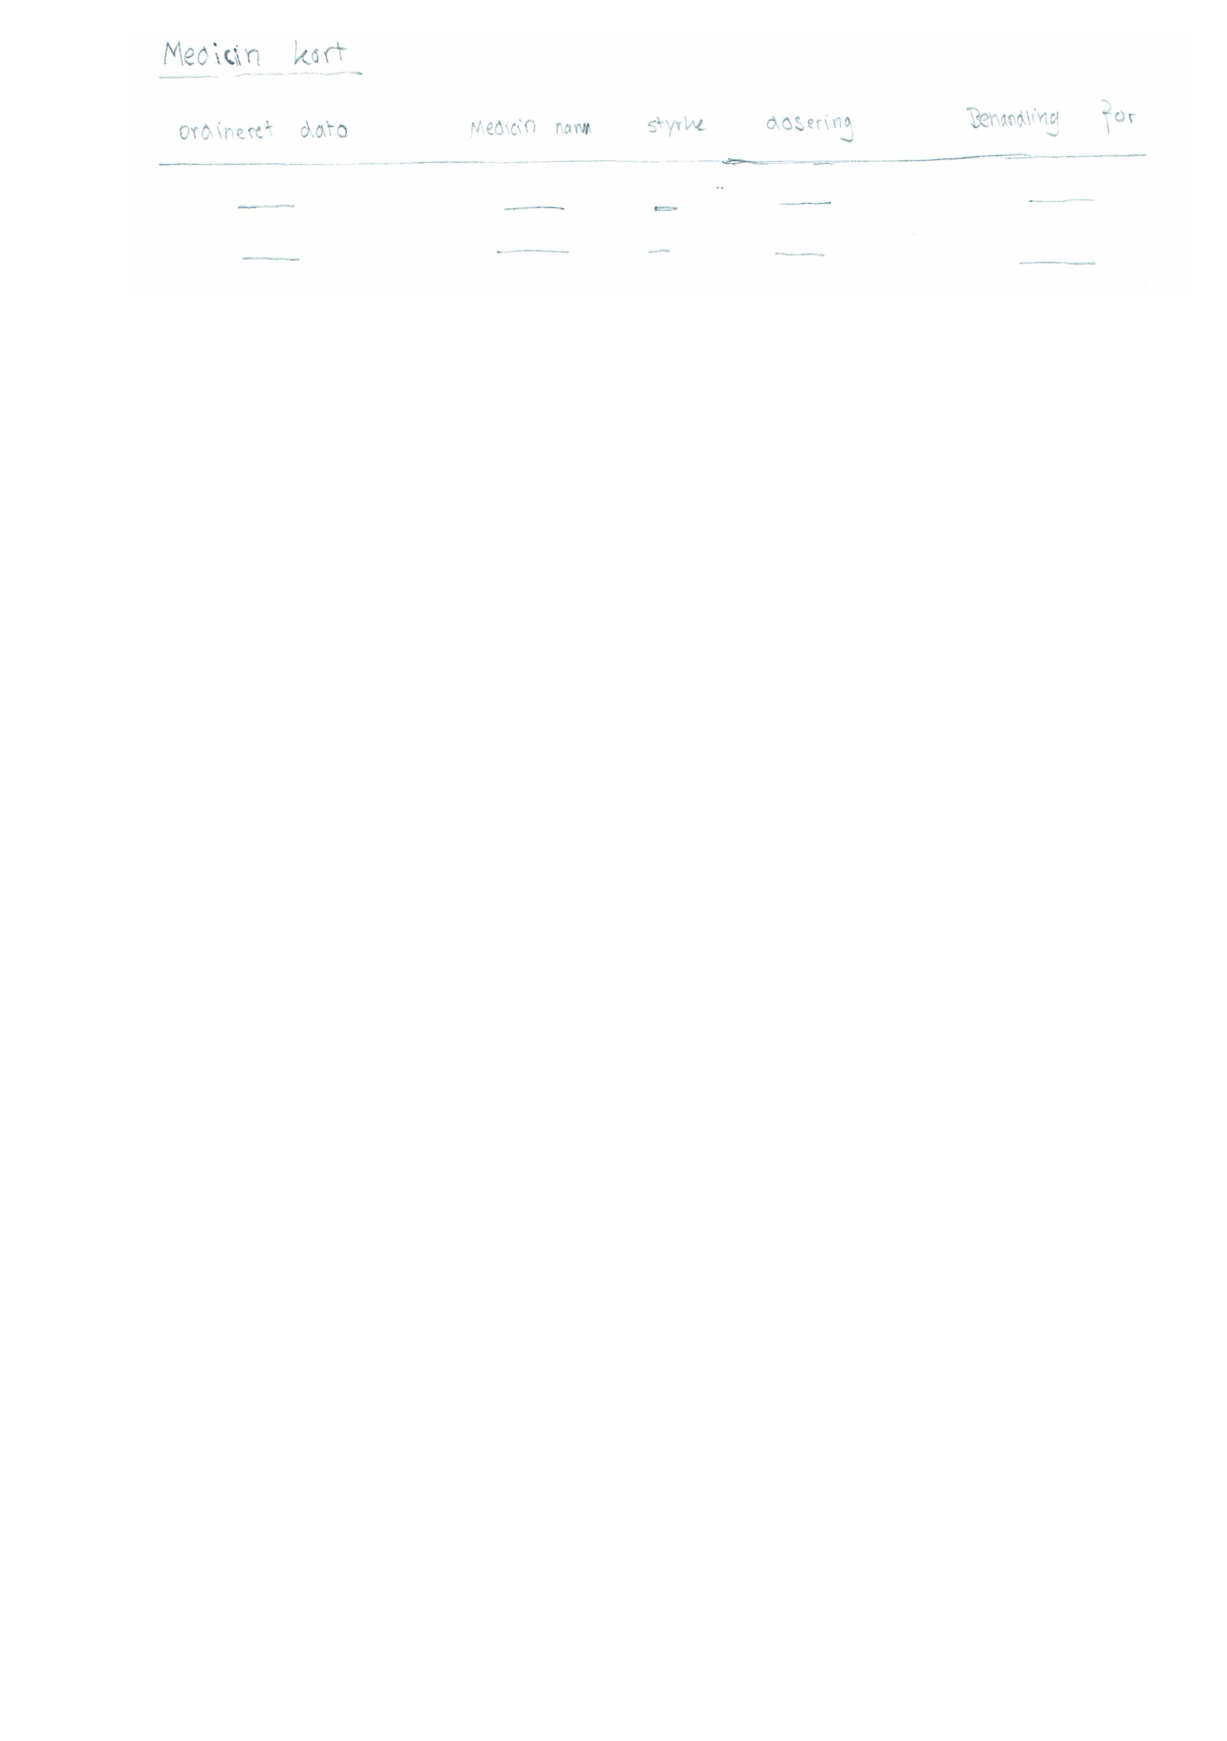
\includegraphics[angle=0, height=0.2\textheight]{Materials/FornyRecept_Medicinkort.pdf}
	\caption{Mock-up for modulet 'Receptfornyelse': Undermenu, 'Medicin kort'}
	\label{fig:Mock-Up}
\end{figure}
\begin{figure}[H]
	\centering
	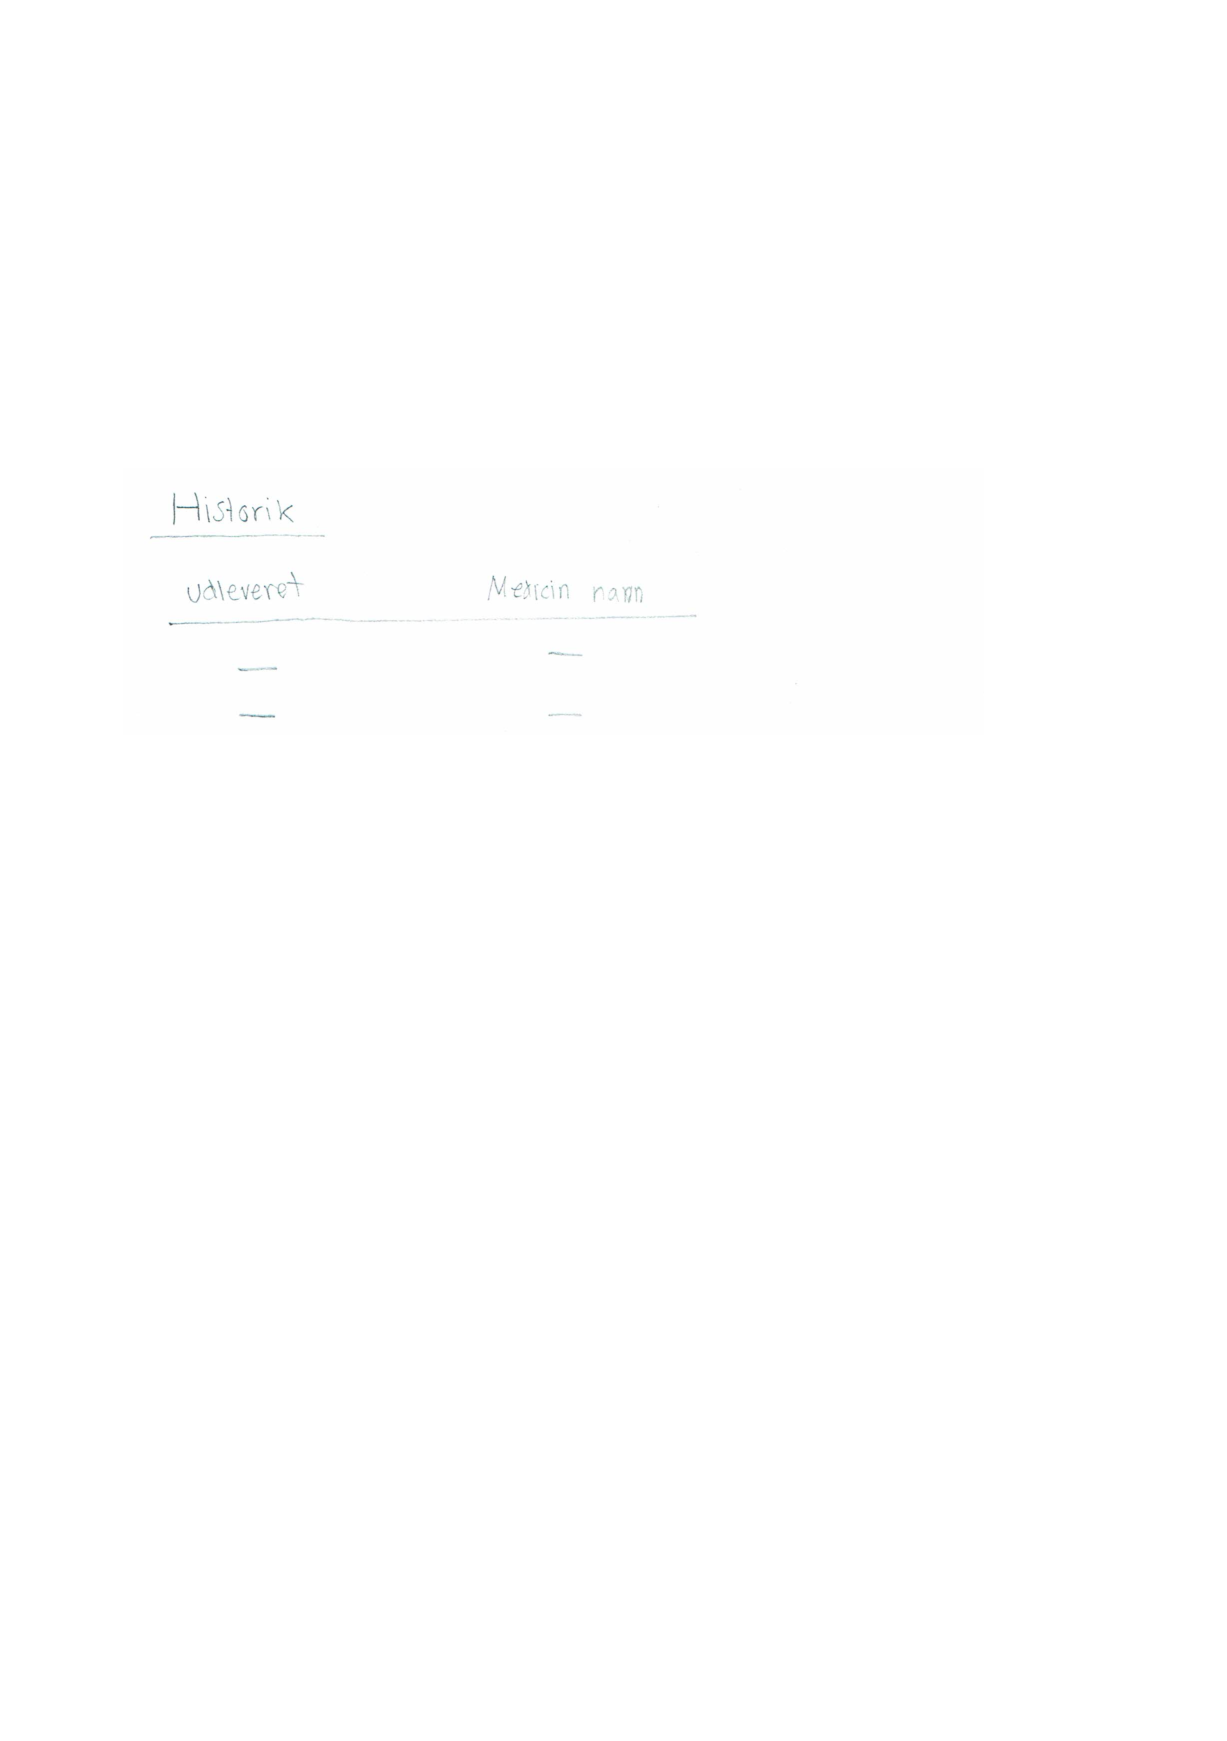
\includegraphics[angle=0, height=0.2\textheight]{Materials/FornyRecept_Historik.pdf}
	\caption{Mock-up for modulet 'Receptfornyelse': Undermenu, 'Historik'}
	\label{fig:Mock-Up}
\end{figure}
% ? - Scenarios
\textbf{Prioritet 2, Samling af al information} \\
Forslag til brugergrænseflade for patienten fremgår af nedenstående Mock-up's:\\
\begin{figure}[H]
	\centering
	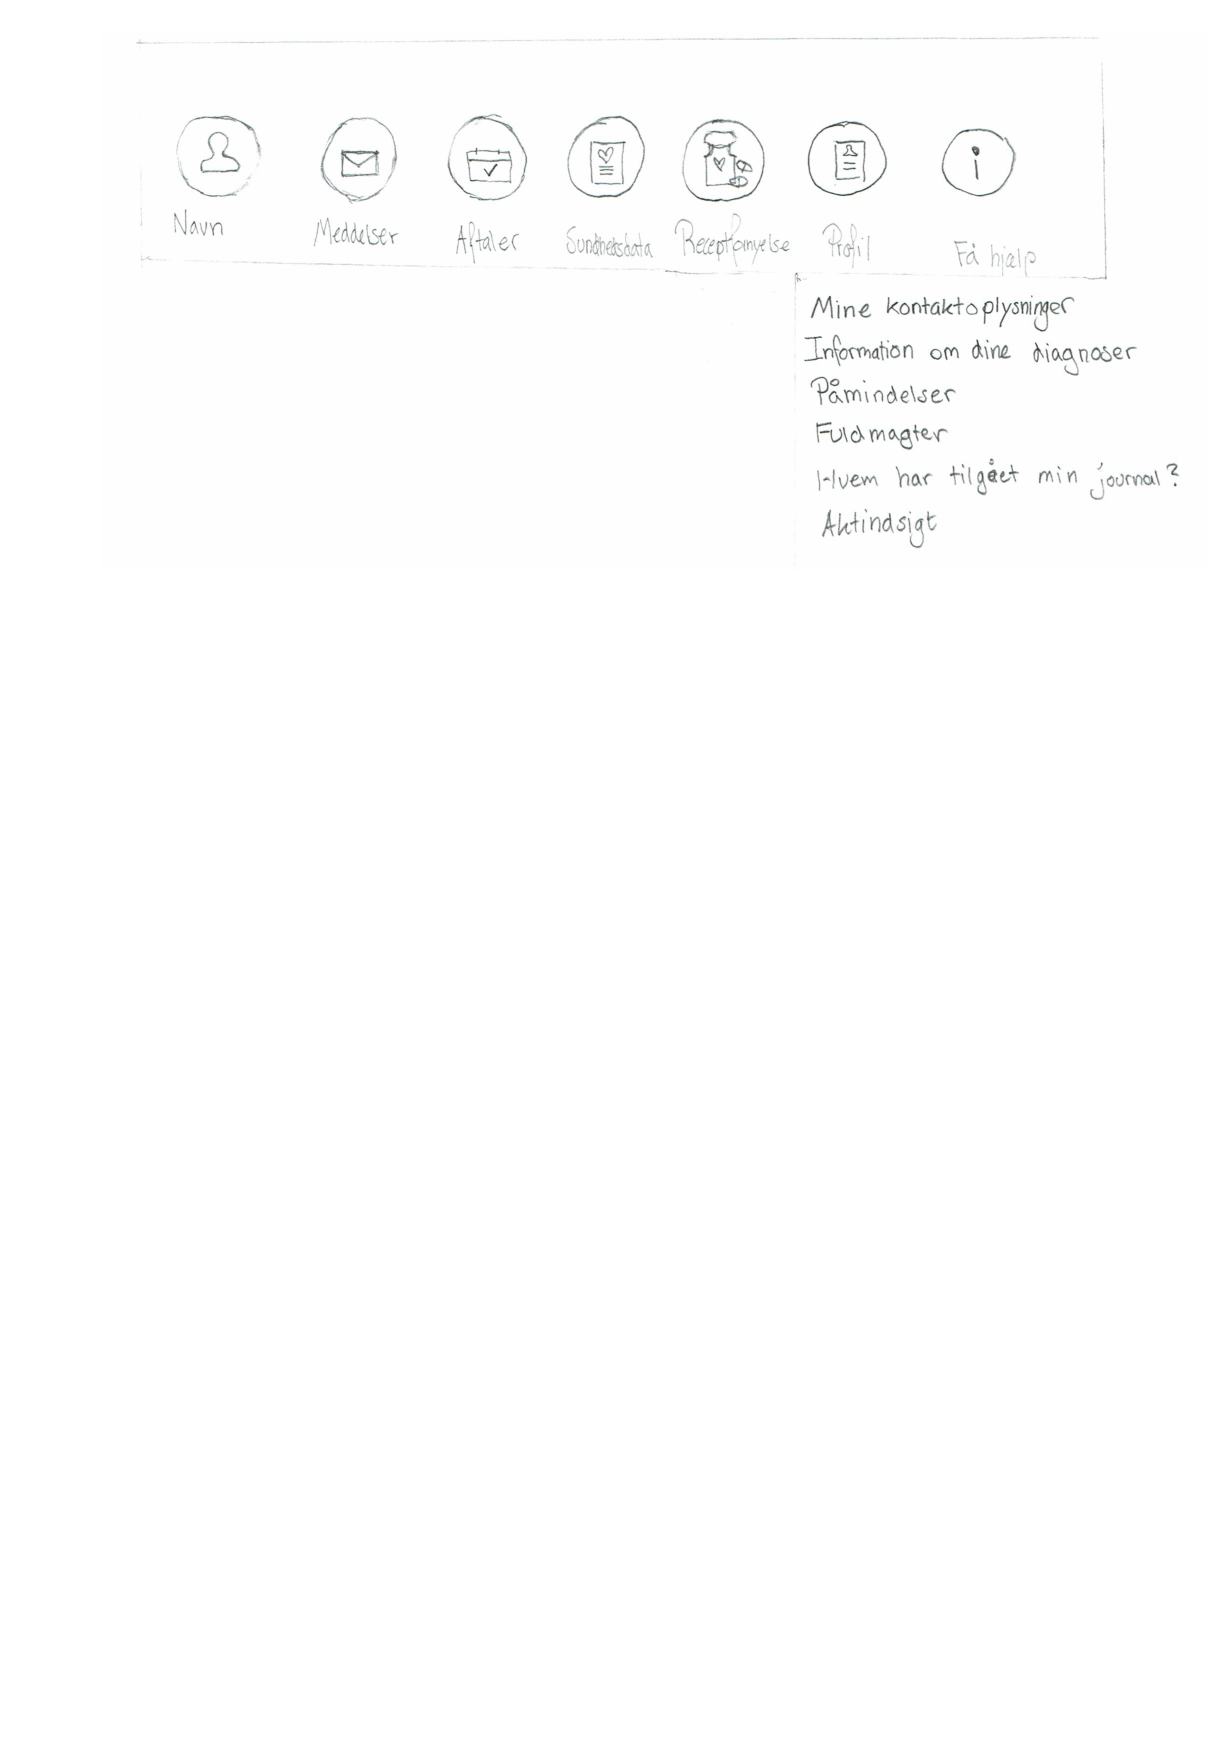
\includegraphics[angle=0, height=0.3\textheight]{Materials/Information_Hovedmenu.pdf}
	\caption{Mock-up for modulet 'Information om dine diagnoser': Hovedmenu, 'Profil'}
	\label{fig:Mock-Up}
\end{figure}
\begin{figure}[H]
	\centering
	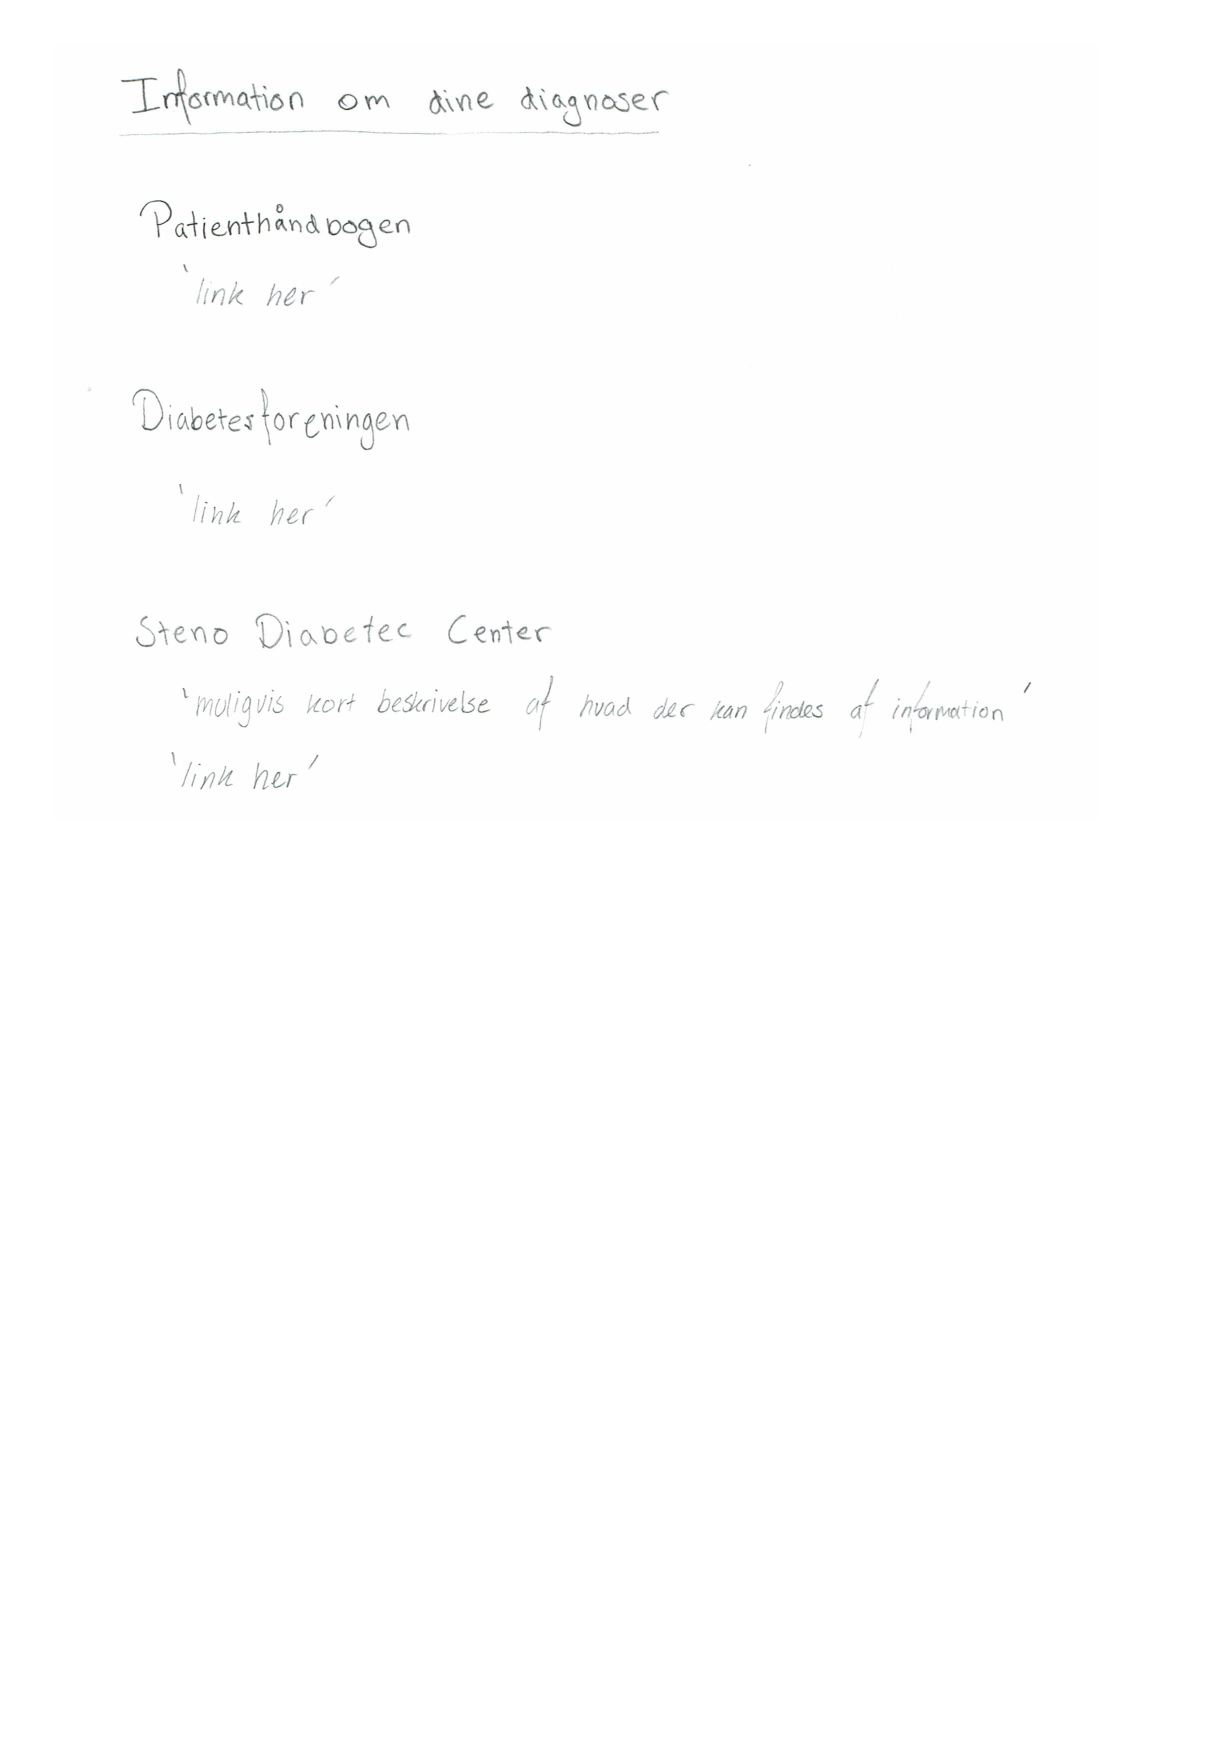
\includegraphics[angle=0, height=0.44\textheight]{Materials/Information.pdf}
	\caption{Mock-up for modulet 'Information om dine diagnoser': Undermenu}
	\label{fig:Mock-Up}
\end{figure}
\textbf{Prioritet 3, Uniforme Prøvesvar} \\
Forslag til brugergrænseflade for patienten fremgår af nedenstående Mock-up's:\\
\begin{figure}[H]
	\centering
	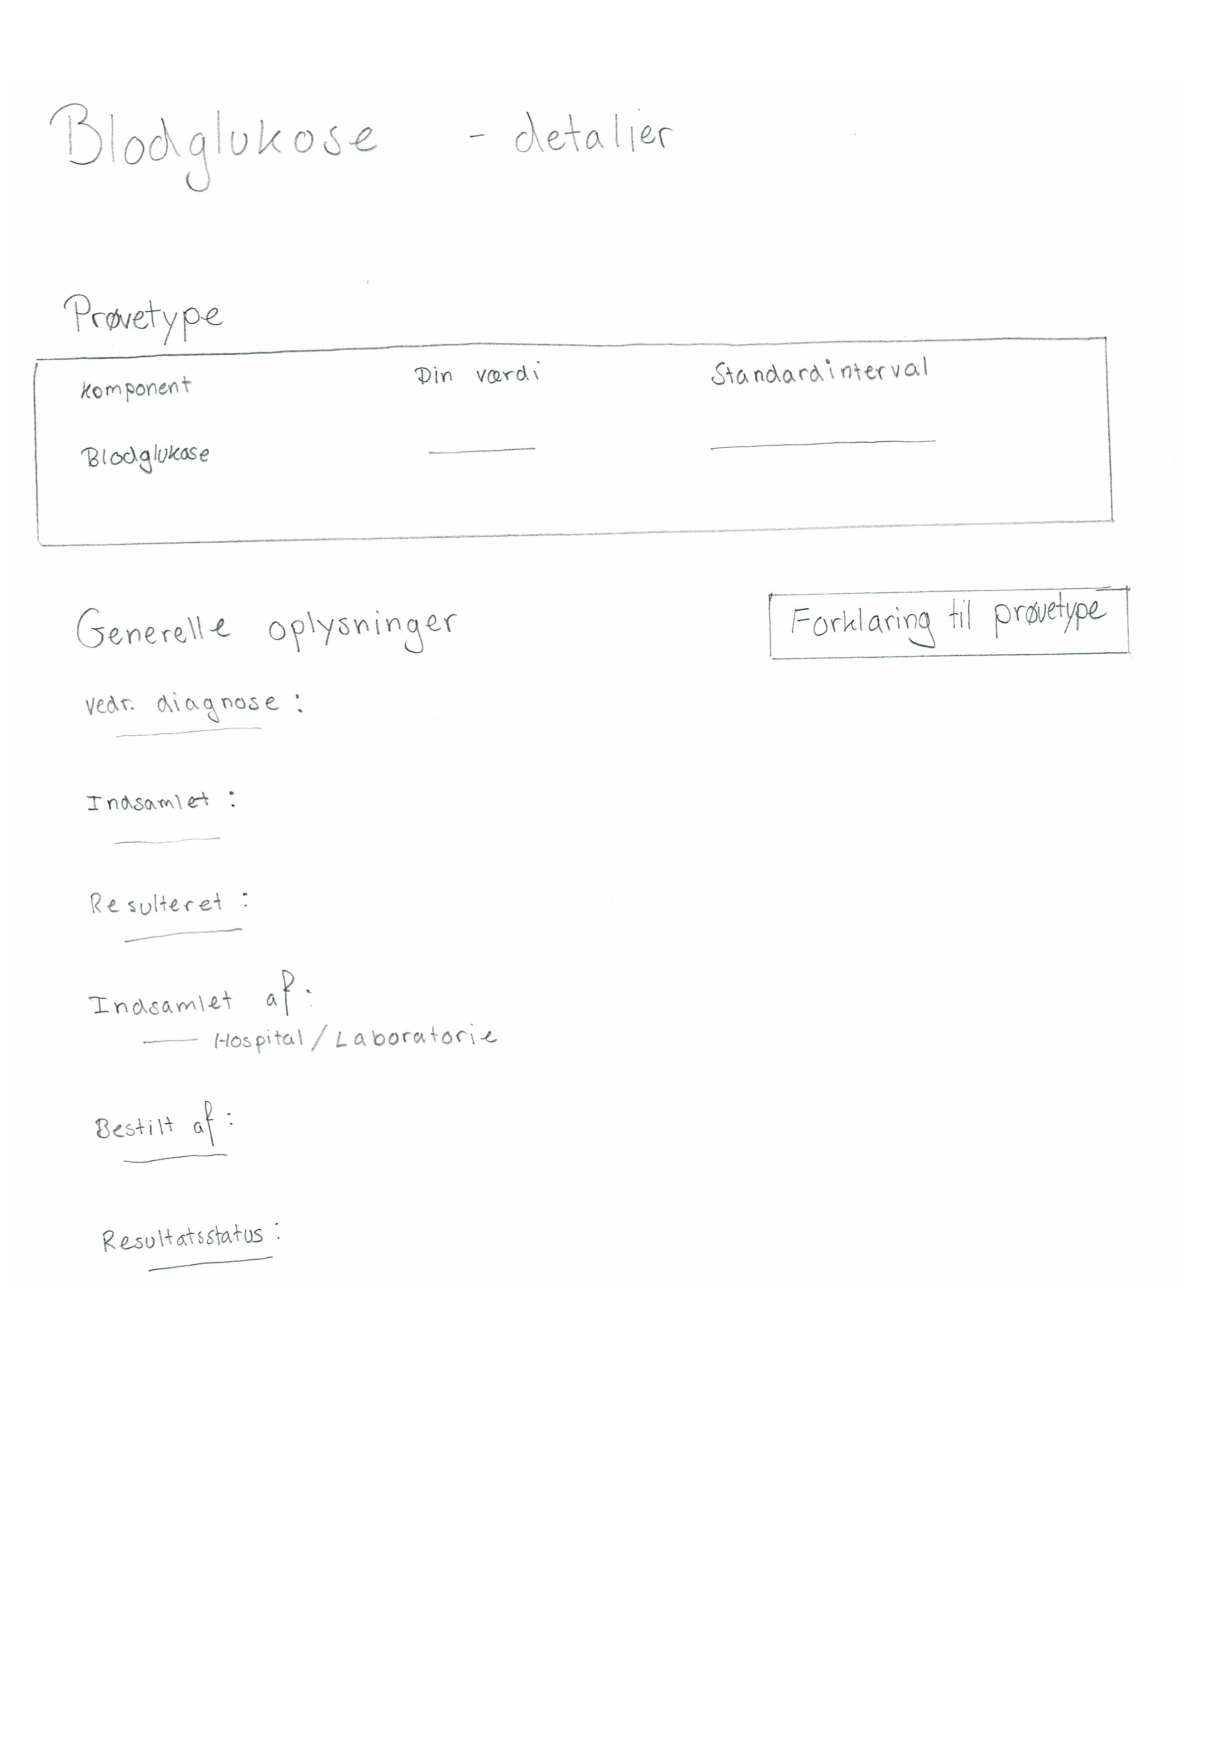
\includegraphics[angle=0, height=0.7\textheight]{Materials/provesvar.pdf}
	\caption{Mock-up for modulet 'Prøvesvar'}
	\label{fig:Mock-Up}
\end{figure}
Når patienten klikker på knappen 'Forklaring til prøvetype' skal der vises en tekst på dansk med forklaringen til prøvetypen. Det kan laves som en pop-up eller ny side.\\

\subsection{Arbejdets organisering} 
Det lykkes desværre ikke for os at få mulighed for at fortage virksomhedsbesøg. \footnote{Dybdeanalyse, afsnit 5 Konsekvensanalyse s. 18} Virksomhedsbesøg ville have givet os mulighed for at observere sundhedspersonalets nuværende arbejdspraksis når patienterne fornyer deres recept via besked funktionen i MinSP og for taget prøver og givet prøvesvar. \\
Vi vil derfor bedre have kunne vurdere hvilken ændringen det betyder i arbejdsorganisering for sundhedspersonalet og arbejdsfordelingen i mellem læge, lægeseerætere, laboranter m.fl.\\
Vi havde også f.eks. haft mulighed for at observere forretningsgange når patienterne bestilte receptfornyelse via sunhed.dk eller en læges eget system, og fået inspiration til vores udvikling af receptfornyelse i MinSP.\\
Vi vil derfor havde haft et bedre grundlag for at vurdere fordele og ulemper for sundhedspersonalet og relationerne i mellem dem, deres arbejdsgange og evt. kvalifikationsbehov ved implementering af vores visioner.\\
Vi har derfor ikke haft den viden som MUST-metodens princip om at arbejdspraksis skal opleves ellers kunne have givet os. 
\\
\\
\textbf{Prioritet 1, Receptfornyelse} \\
En automatisk receptfornyelse vil muligvis ændre arbejdsgangen for sundhedspersonalet. \\ 
Lægen skal fortsat stadigvæk tjekke, at ordineringen er korrekt i forhold til journalen, men at læge-sekretæren slipper for at skrive besked tilbage til patienten, da patienten nu selv kan se forløbet i statuslinjen.
%
\\\\
\textbf{Prioritet 2, Samling af al information} \\
Hvis funktionaliteten implementeres via links, som forslået, vil der ikke være nogen ændringer til arbejdsgange og arbejdets organisering. \\
Hvis ikke funktionaliteten implementeres via links, men som en ny-udviklet informationside, er det sundhedspersonalet der skal skrive alt informationen / optage videoer mv og siden vil skulle vedligeholdes af sundhedspersonalet, så det ville være en ekstra opgave, som sundhedspersonalet (læger, diætister og sygeplejeskær m.fl.) herved bliver pålagt.
\\\\
\textbf{Prioritet 3, Uniforme Prøvesvar} \\
Implementering af denne funktionalitet vil give ekstra arbejde for lægesekretæren eller laboratorie medarbejdere i forhold til indrapporteringen af prøvesvar, da der vil være flere informationer (navn på sted hvor prøven er taget og navn på diagnose), der skal indtastes, end med nuværende løsning. Der vil forinden være ekstra arbejde for lægen, da det er denne, der skal informere laboratorie-personale eller lægesekretær om hvilken diagnose de enkle prøvesvar vedrører.\\
Der skal tages stilling til hvor i organisationen indrapporteringen skal foretages.
\subsection{Kvalifikationsbehov}
\textbf{Prioritet 1, Receptfornyelse} \\
Receptfornyelses funktionaliteten vil ikke kræve nogen større oplæring af sundhedspersonalet, kun en introduktion til hvordan den nye funktionalitet fungerer.
\\\\
\textbf{Prioritet 2, Samling af al information} \\
Hvis funktionaliteten implementeres via links, vil det ikke kræve nogen oplæring af sundhedspersonalet.
\\\\
\textbf{Prioritet 3, Uniforme Prøvesvar} \\
Vores vurdering er, at ændringerne ikke kræver ekstra kvalifikationer, da ændringen for sundhedspersonalet består i data-indtastning, som de allerede er bekendt med.